\startblue
Throughout the development of this thesis, the establishment of deep learning as a strategy where computers learn through representation of patterns at varying degrees of complexity has been an underlying theme.  It was also emphasised how this is achieved by internal layer-wise encapsulations. Structures discussed in Chapter \ref{ch2litrev}, such as layer-wise stacking of neural network type architectures such as the \acrlong{rbm} (\acrshort{rbm}) \acrlong{dbn} (\acrshort{dbn}) were used to implement such representations.  

In this chapter, the end-to-end Bi-directional Recurrent Neural Network model is described.  \acrshort{birnn} for speech recognition tasks is  employed here as opposed to regular \acrshort{rnn}s or \acrshort{dbm}s mentioned above in the preceding paragraph.  Use of \acrshort{birnn}s is attributed to the contextual nature of speech.  Furthermore, we saw in the preceding Chapter how deep stacking of \acrshort{gru}s outperform single-layer \acrshort{rnn}s for extended sequences. That is to say, words in a sentence or paragraph are contextual to the sentence/paragraph over particularly long sequences are captured better by the GRU architecture.  In addition, \acrshort{birnn}'s have a forward and backward \acrshort{rnn} and these give the neural network the ability to analyse (look-up) the words from the backward RNN not currently seen by the forward RNN in the sentence succinctly giving the BiRNN parameters a contextual feature \citep{graves2006connectionist}.  

This chapter, however, first discusses speech features developed by making use of the deep scattering convolution networks \acrshort{dsn}.  The \acrshort{dsn}s are used as inputs to the end-to-end model.  Two end-to-end networks are then described.  The core \acrshort{birnn} network and a second \acrshort{birnn} network augmented with an RNN-transducer and an attention mechanism. A formal presentation of the speech neural network model parameters and architecture is given and the decoding algorithm is also detailed in sections contained within this chapter.  Finally, the results are presented and the findings from the model results discussed.\stopblue

\section{Deep Scattering Features}\label{sec_c7_wparams}
\textcolor{blue}{In Chapter 4, we derived a fast wavelet transform from a low pass filter and a high pass filter.  The speech features used for the BiRNN is obtained from successive wavelet-modulus operations of a deep scattering network 2 layers deep.  This 2-layer \acrshort{dsn} comprises a first-order scatter transform. The wavelet modulus operator is derived from the combination of a low pass filter and a band pass filter}.  Hyper parameters of the system included the window period for each sampled sub section, $T$;  The Q-band value for the band pass filter and the number of wavelets $J$ at each scattering layer for the total number of layers, $M=2$.

\textcolor{blue}{For the second end-to-end architecture involving a transducer with attention mechanism, a period of $$T=2^16$$ is used to capture a window of 4 seconds for audio signals sampled at 16000Hz. The same Q-band parameters are used.}

The matlab scatnet toolbox \citep{anden2014scatnet}, used to determine the scatter coefficient features for this research, provides optimal values for hyper parameters for audio signal processing into scatter features.  In this regime the value for the hyper parameter $T=512$ samples per window. This corresponds to a window of $50$ milliseconds for the audio signals sampled at $8000 Hz$.  For the first scattering layer the $Q$-band parameter was $Q=8$ and the second scattering layer took the value  $Q=1$.  Finally $J$ is pre-calculated based on the value of $T$.  These after Scat-Net processing produce a feature-vector having \textcolor{red}{$165$}  dimensions.  These feature vectors in turn are used as inputs to the bi-direction neural network model whose architecture is described in  succeeding sections.

\section{CTC-BiRNN Architecture}
The core of the system is a bidirectional recurrent neural network (BiRNN) trained to ingest scatter coefficients described in the previous section, in order to generate English text transcriptions.  An end-to-end system therefore specifies that utterances $x$ and the corresponding label $y$ be sampled from a training set such that the sample $S = {(x^{(1)}, y^{(1)}), (x^{(2)}, y^{(2)}), . . .}$.   In our end-to-end model, each utterance, $x^{(i)}$ is a processed feature vector consisting of $165$ dimensions.  Recall, every window passes through a scattering transform to yield an input of vector of $p=165$ features; consequently,   $x^{(i)}_{t,p}$ denotes the $p$-th feature in a scatter transform at time $t$.  

GPU training of the speech model architecture developed above was conducted using Mozilla deepspeech \citep{mozilla/deepspeech_2019} CTC bi-directional RNN implementation along with the accompanying Mozilla Common voice dataset  \citep{mozilla_2019}.  The Common Voice Dataset project consists of voice samples in short recordings approximately $4$ seconds each.  The complete dataset is about $250$ hours of recording divided into training, test and development subsets.  The BiRNN, given the input sequence, $x$, outputs a sequence of probabilities $y_t=\mathbb{P}(c_t|x)$,  where $c_t \in a,b,c,\dots,z,space,apostrophe,blank$. 

The actual architecture of our core Bi-RNN is similar to the deepspeech system described in \cite{hannun2014deep}. This structure constitutes 5 hidden layers and one output layer.  The first three layers are regular DNNs followed by a bi-directional recurrent layer. As such, the output of the first three layers are computed by:
\begin{equation}
    h^{(l)}_t = g(W^{(l)} h^{(l−1)}_t + b^{(l)})\label{ch06_01_l1-3}
\end{equation}

$g(\cdot) = min\{max\{0,z\},20\}$  is the clipped rectified linear unit and $W^{(l)},b^{(l)}$ are weight matrix and bias parameters for layer  as described in sections \ref{dnn} and \ref{deepspeech} respectively.

It was shown in chapter \ref{ch3RNN} the recurrent layer comprise a forward and backward RNNs whose equations are repeated here for reference
\begin{equation}
    h^{(f)}_t = g(W^{(4)} h^{(3)}_t + W^{(f)}_r h^{(f)}_{t−1} + b^{(4)})
    \label{ch06_02_fwd}
\end{equation}
\begin{equation}
h^{(b)}_t = g(W^{(4)} h^{(3)}_t + W^{(b)}_r h^{(b)}_{t+1} + b^{(4)})    \label{ch06_03_bwd}
\end{equation}

Consequently, $h^{(f)}$ is the sequential computation from $t=1$ to $t=T^{(i)}$ for the $i$-th utterance and $h^{(b)}$ is the reverse computation from $t=T^{(i)}$ to $t=1$.  In addition the output from layer five is summarily given as the combined outputs from the recurrent layer:
\begin{equation}
h^{(5)} = g(W^{(5)} h^{(4)} + b^{(5)})    \label{ch06_04_l5}
\end{equation}
where $h^{(4)} = h^{(f)} + h^{(b)}$. The output of the Bi-RNN on layer 6 is a standard soft-max layer that outputs a predicted character over probabilities for each time slice $t$ and character $k$ in the alphabet:
\begin{equation}
h^{(6)}_{t,k} = \hat{y}_{t,k} \equiv \mathbb{P}(c_t = k \mid x) = \frac{\exp{ \left( (W^{(6)} h^{(5)}_t)_k + b^{(6)}_k \right)}}{\sum_j \exp{\left( (W^{(6)} h^{(5)}_t)_j + b^{(6)}_j \right)}})    \label{ch06_05_l6}
\end{equation}

$b^{(6)}_k$ takes on the -th bias and $(W^{(6)} h^{(5)}_t)_k$ is the matrix product of the $k$-th element.  The error of the outputs are then computed using the CTC loss function \cite{graves_2014} as described in chapter \ref{ch3RNN}.  A summary of our model is illustrated in Figure \ref{fig_6_1_ctc_scatter}.
\begin{figure}
\centering
  % Requires \usepackage{graphicx}
  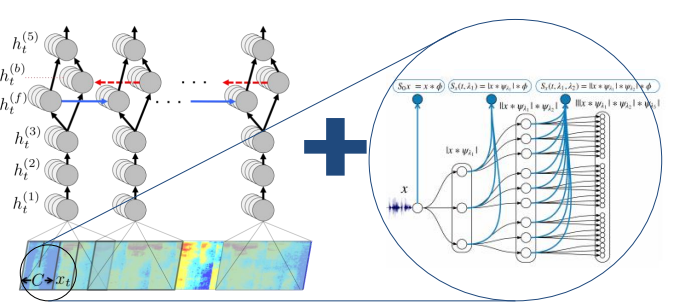
\includegraphics[width=14cm]{thesis/images/ctc_scatter.png}\\
  \caption{Deep scattering Bi-RNN Model} \label{fig_6_1_ctc_scatter}
\end{figure}

\section{CTC Decoding}

In chapter three the CTC loss function algorithm was established as being able to maximise the probability of two cases.  The first case of transiting to a blank and the second case of transiting to a non blank.  In this section, this concept is used to enable decoding of the network output from posterior distribution output to character sequences which can be measured against a reference transcription using either character error rate (CER) or word error rate (WER).

Recall, all the output symbols are in the alphabet $\Sigma$ and augmented with the blank symbol. The posterior output of the CTC network is the probability of the symbol given the speech feature input $p(c|x_t)$ at time $t$ for $t=1,\dots,T$ and $T$ is the length of the input sequence.  Also recall two further sets of probabilities also being maintained by the model are the probability of a blank character $p_b$ and that of a non blank character $p_{nb}$.

Several strategies have been employed to obtain a translation string from the output of the deep neural network.  The prefix beam search employed by the CTC decoder of this research is derived from an initial greedy approximation, where at each time step determine the argument that maximises the  probability $p(c|x_t)$ at each time step. Let $C=(c_1,\dots,c_T$ be the character string then, the greedy approach has 
\begin{equation}
    c_t=arg\max_{c\in\Sigma}p(c|x_t)
\end{equation}
However, this simple approximation is unable to collapse repeating sequences and remove blank symbols. In addition, the approximation is unable to include the constraint of a lexicon or language model.

The prefix beam search algorithm \cite{hannun2014first} adopted in this work incorporates a language model derived from a lexicon in addition to keeping track of the various likelihoods used for decoding.  For the language model constraint, the transcription $W$ is recovered from acoustic input $X$ at time $t$ by choosing the word which maximising the posterior probability:
\begin{equation}
W_i=arg\max_{W_i \in \Sigma_W} p_{net}(W;X)p_{lm}(W)
\label{eqn_c6_decoder01}
\end{equation}
In equation \ref{eqn_c6_decoder01}, the Bayes product of language model prior $p_{lm}$ and the network output $p_{net}$ are utilised to maximise the probability of a particular character-word sequence in the lexicon given by $\Sigma_W$.  The overall calculation used to derive the final posterior distribution includes word insertion factors ($\alpha$ and $\beta$) used to balance the highly constrained n-gram language model.

The second strategy adopted by the prefix beam search which improves the decoding algorithm is the beam search strategy.  With this approach, the search maintains all possible paths; however, it retains only $k$ number paths which maximise the output sequence probability.  Improvements gained with this method are seen when certain maximal paths are made obsolete owing to new information derived from the multiple paths in being maintained in memory. 

The recursive prefix beam search algorithm illustrated in Figure \ref{fig_c6_decoder01} attempts to find the string formulated in equation \ref{eqn_c6_decoder01}.  Two sets prefixes $A_{prev}$ and $A_{nxet}$ are initialised, such that at $A_{nxet}$ maintains the prefixes in the current time-step while $A_{prev}$ maintains only $k$-prefixes from the previous time-step.  Note that at the end of each time step $A_{prev}$ is updated with only -most probable prefixes from $A_{nxet}$. Therefore while,  $A_{nxet}$ contains all the possible new paths from based on $A_{prev}$ as a Cartesian product of $A_{prev} \times \Sigma \in \mathcal{Z}^k\times\mathcal{Z}^{|\Sigma|}$ where $|\Sigma|$ is the length of $\Sigma$. The probabilities of each prefix obtained at each time step are the sum of the probability of non-blank plus the probability of a blank symbol.
\begin{sidewaysfigure}[ht]
    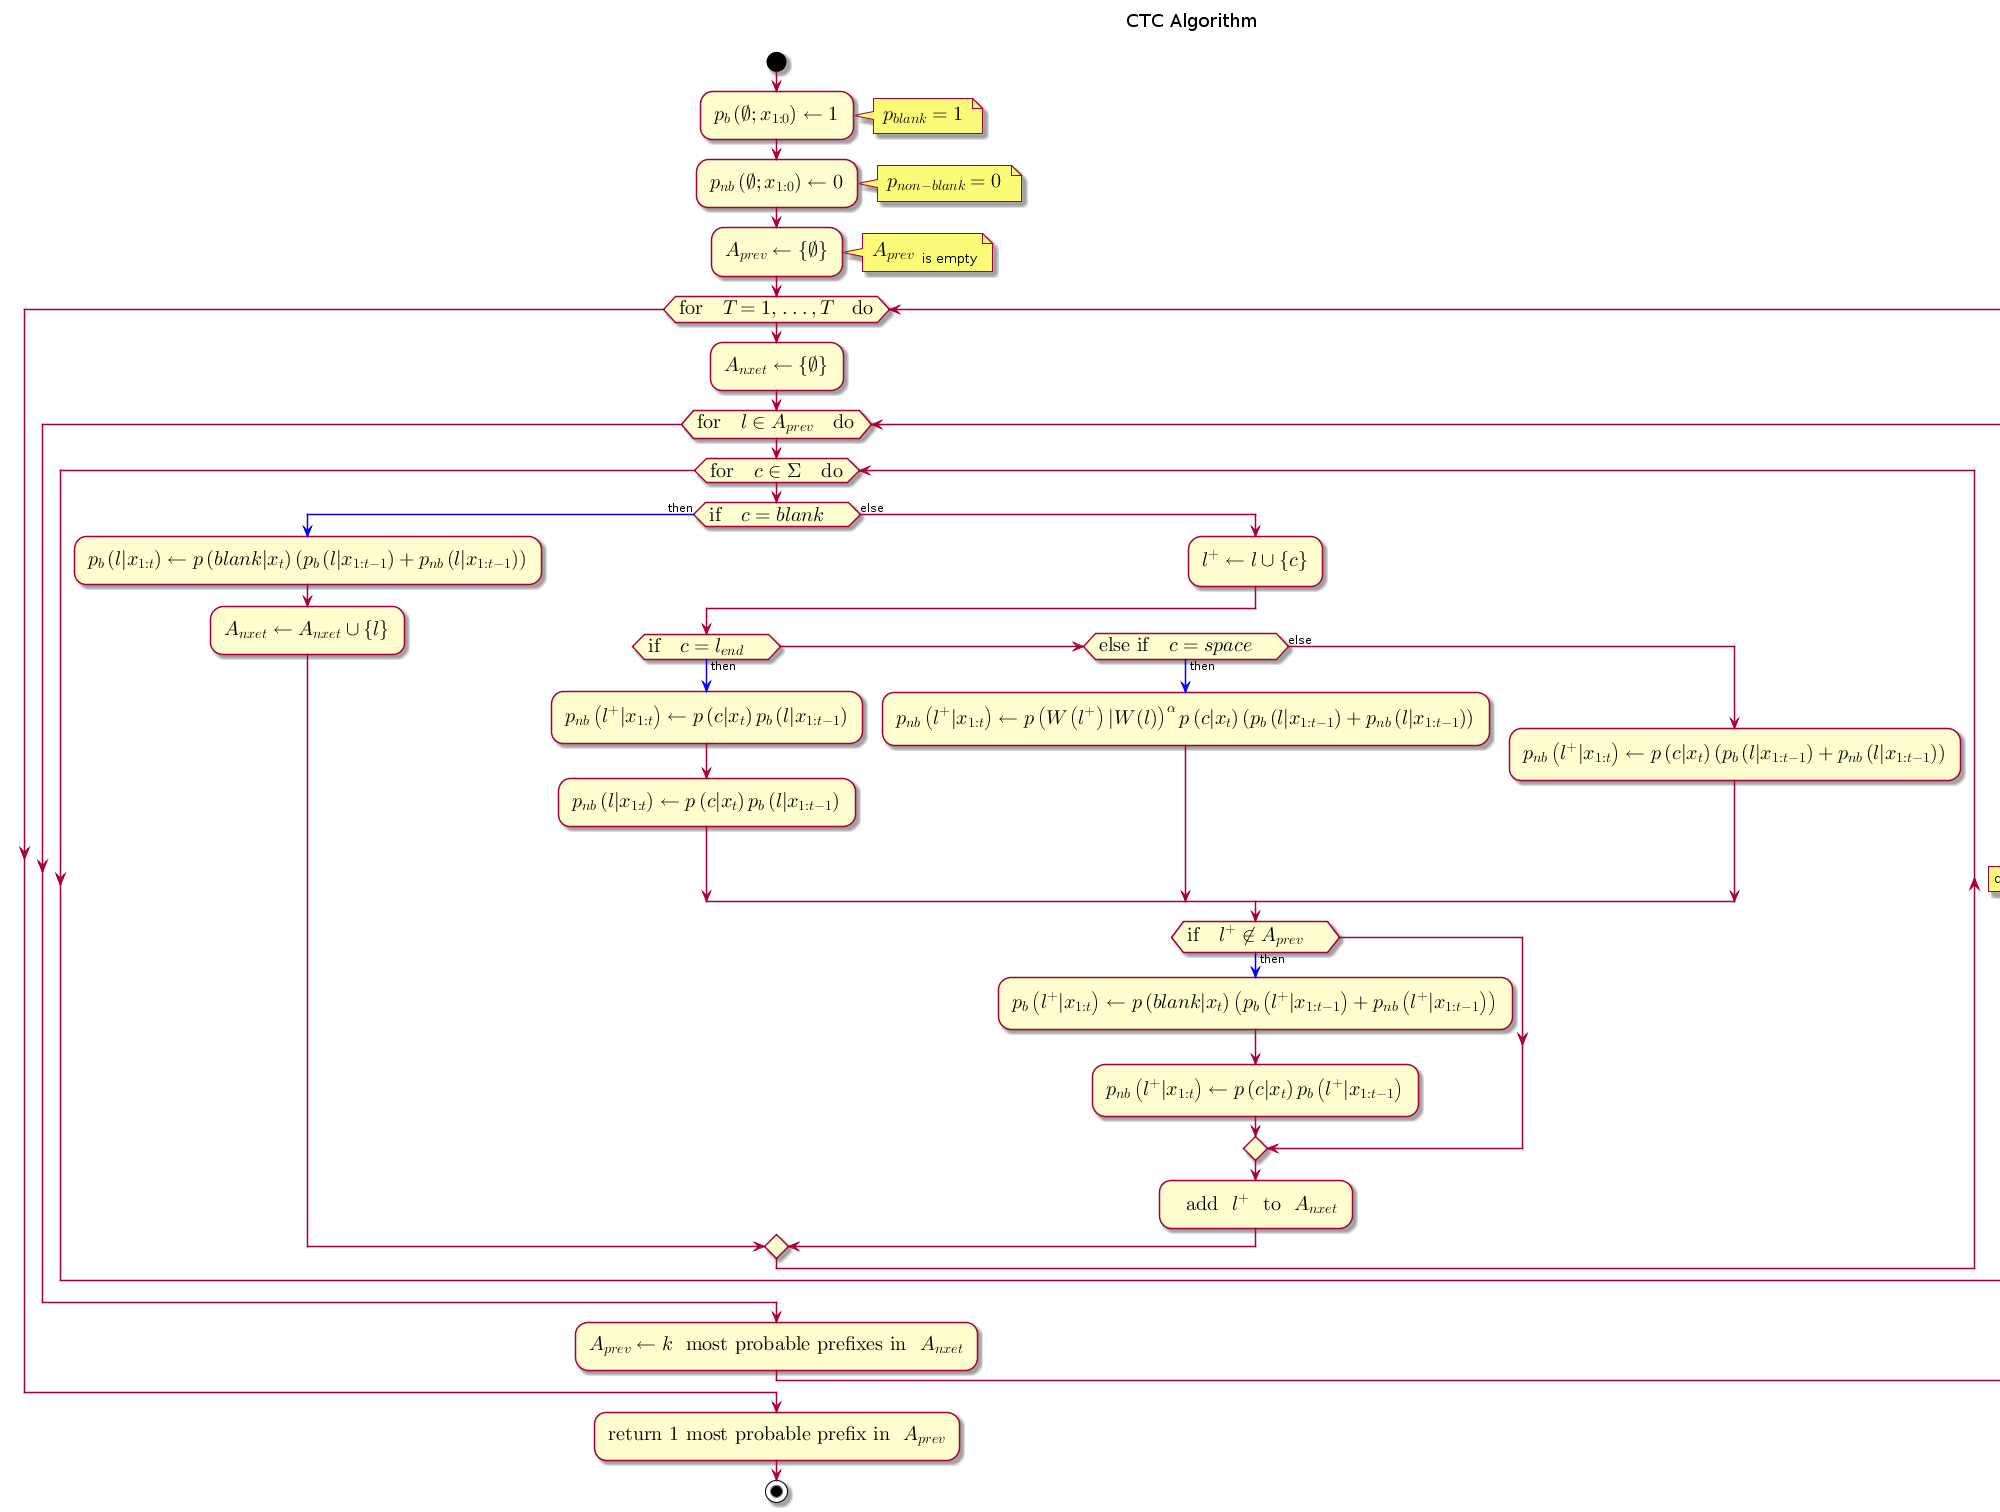
\includegraphics[width=22cm]{ctc}
    \caption{Prefix beam search algorithm}
    \label{fig_c6_decoder01}
\end{sidewaysfigure}

At every  time step and for every prefix $\ell$ currently in $A_{prev}$, a character from the alphabet $\Sigma$ is presented to the prefix. The prefix is only extended only when the presented symbol is not a blank or a space. $A_{nxet}$ and $A_{prev}$ maintain a list of active prefixes at the previous time step and proposed prefixes at the next time step respectively, The prefix probability is given by multiplying the word insertion term by the sum of the blank and non-blank symbol probabilities.
\begin{equation}
p(\ell|x_{1:t})=(p_{nb}(\ell|x_{1:t})+p_b(\ell|x_{1:t}))|W(\ell)|^\beta
\label{eqn_c6_decoder03}
\end{equation}

$W(\cdot)$ is obtained by segmenting all the characters in the sequence with the space-character symbol and truncating any characters trailing the  set of words in the sequence.  The prefix distribution however varies slightly depending on network output character being presented.

$\ell_{end}$ is the variable representing the last symbol in the prefix sequence in $A_{prev}$. If the symbol presented is the same as $\ell_{end}$ then the probability of a non-blank symbol,$p_{nb}=0$ . If the symbol being presented is blank then we do not extend the prefix.  Finally, if the symbol being presented is a space then we invoke the language model as follows
\begin{equation}
p(\ell^+|x_{1:t})=p(W(\ell^+)|W(\ell))^\alpha(p_{nb}(\ell|x_{1:t})+p_b(\ell|x_{1:t}))|W(\ell)|^\beta
\label{eqn_c6_decoder03}
\end{equation}

Note that $p(W(\ell^+)|W(\ell))$ is set to $0$ if the current word $W(\ell^+)$ is not in the lexicon. This becomes a constraint to enforce all character strings to consist only of words in the lexicon.  Furthermore,  $p(W(\ell^+)|W(\ell))$ is extended to include all the character sequences representing number of words considered by the n-gram language model by constituting the last $n-1$ words in character sequence $W(\ell)$.

\begin{figure}
\centering
  % Requires \usepackage{graphicx}
  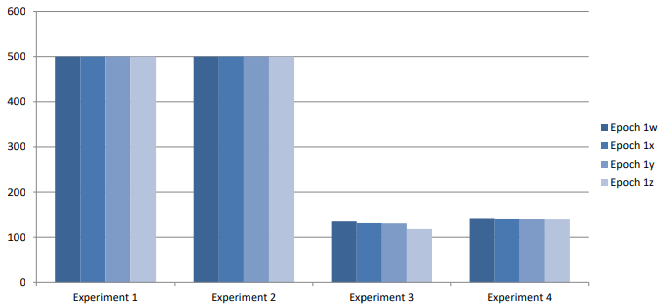
\includegraphics[width=14cm]{thesis/images/res00.PNG}\\
  \caption{Training Loss, where $w<x<y<z$ are taken arbitrarily across the
total number of epochs} \label{fig_6_2_loss}
\end{figure}

\section{Model Hyper parameters}
The hidden layer matrix for each layer comprised 1024 hidden units (6.6M free parameters).  The weights are initialised from a uniform random distribution having a standard deviation of 0.046875.  The Adam optimisation algorithm \citep{kingma2014adam} was used with initial learning rate of, and a momentum of 0.95 was deployed to optimise the learning rate.

The network was trained for a total of five to fifty epochs over the training set for experiments conducted. The training time for Python GPU implementation is shown in Table \ref{tab_c6_01_training}.  For decoding with prefix search we use a beam size of $200$ and cross-validated with a held-out set to find optimal settings for the parameters $\alpha$ and $\beta$. Figure \ref{fig_6_3_wer} shows word error rates for various GPU configurations and audio data-set sizes.

\section{BiRNN with Transducer+Attention end-to-end Architecture}
The end-to-end architecture at the core of ESPNet is the CTC-Transformer+Attention Transducer model.  Together these two architectures achieve joint multi-objective speech training and decoding.  The CTC-Transformer model is based on a Bi-RNN similar to what is obtainable in the DeepSpeech model.  The attention transducer model is further explained in Chapter \ref{ch8further}.  There are up to 11 variants of Attention networks implemented in ESPNet, however, the results of the ESPNet experiment performed was determined from the model described in \cite{chorowski2015attention}.  Moreover, the multi-objective training was performed with equal weights on both the CTC-transformer and the Attention-Transducer.  Finally the system was trained for 20 epochs only.

With this minimal default setting, the test set had a final recognition score of 9.5\% character error rate (CER).  The next Chapter discusses how the baseline can be scaled and remodelled for integrating scattering features.

\section{Attention-based Models}
The objective of attention-based networks highlighted by  \cite{vaswani2017attention} is to reduce sequential computation while attaining hidden representation across arbitrary lengths of sequential input. Mechanisms which have been deployed to achieve this includes a combination of convolutional and recurrent schemes \citep{kaiser2016can,kalchbrenner2016neural, gehring2017convolutional}. \cite{vaswani2017attention} introduces a transduction model known as a Transformer based on self attention network with the ability to compute long term dependencies while eliminating sequence aligned RNN and convolutional architectures.

Self attention is a network that intrinsically reduces the need for intensive resource training.  \cite{vaswani2017attention} reports that state of the art BLEU score of 41.0 having used a small fraction of training resources.  While GANs might not be attractive for low resource speech recognition, they still remain an important tool for verification of the output of other networks.  At the same time self attention networks can help to reduce the resource requirements of GANs when used within the context of a GAN.

As a study to further this thesis, these networks are likely candidates for network training using scatter features as input discriminatory functions.  Attention based networks as a means to reduce training resources required, while GANs can be used as a means to generate training data.

\section{Joint Training with ESPNet}
Chapter \ref{ch6_speech} has already seen promising results based on preliminary experiments using the ESPNet model.  This model does fulfil major objectives outlined by this research. The inclusion of Attention-based models and the warp-CTC decoder implemented in ESPNet ensures faster convergence and ultimately faster time to train, in addition to the end-to-end architecture presented by ESPNet. The next step required for a further study is an integration of scattering features into ESPNet.  This scattering features implementation is the subject of a paper publication immediately sought after based on this work.  The features of ESPNet include state-of-the-art end-to-end architectures including variants of Attention-Transducers and CTC-decoders.  Using a weighting function  one can control how much bias either the CTC-Transform or the Attention-Transducer will get during training.  The joint training helps to improve robustness as well as achieve fast convergence.
\begin{equation}
    \mathcal{L}=\alpha\mathcal{L}^{ctc}+(1-\alpha)\mathacal{L}^{att}
    \label{eqn_c7_esp00}
\end{equation}
At the same time joint decoding of labels is integrated with the character based RNN-language modelling. The log probability of the RNNLM-integrated decoding of character labels is as follows
\begin{equation}
    \log p(y_n|y_{1:n−1},\mathbf{h}_{1:T‘})=\log p^{hyp}(y_n|y_{1:n−1},\mathbf{h}_{1:T‘})+\beta\log p^{lm}(y_n|y_{1:n−1})
    \label{eqn_c7_esp01}
\end{equation}
Where joint decoding, $\log p^{hyp}(y_n|y_{1:n−1},\mathbf{h}_{1:T‘})$ is given by
\begin{equation}
    \log p^{hyp}(y_n|y_{1:n−1},\mathbf{h}_{1:T‘})\\
    & = \alpha\log p^{ctc}(y_n|y_{1:n-1},\mathbf{h}_{1:T'})+(1-\alpha)\log p^{att}(y_n|y_{1:n-1},\mathbf{h}_{1:T'})
\end{equation}
Furthermore, multi-channel training integrates noise robust and far-field speech recognition tasks which can accommodate joint 83-dimension MFCC and scatter transform training in addition to speech enhancement features such as beam forming and STFT masking \cite{ochiai2017multichannel}. Both single and multi-channel scatter transform features are proposed as subjects in the future paper publication. 

\section{Model Baseline}
The study by \cite{hannun2014first} reported successful character error rate (CER)  using deep neural network (DNN), recurrent deep neural network with only forward temporal connections (RDNN), and also bi-directional recurrent neural networks (BRDNN). The models used in this their study had 5 hidden layers having either 1,824 or 2,048 hidden units in each hidden layer.  For a baseline, the model produced by the Mozilla DeepSpeech team was adopted.  This model had a similar architecture with 5 hidden units and 2048 hidden units and was trained on the Librespeech corpus and the common voice data corpora \citep{panayotov2015librispeech, mozilla/deepspeech_2019}.

Word Error Rates by this model were optimised after 75 epochs, learning rate of 0.0001 and a dropout rate of 15\%.  In addition, the language model hyper parameters for alpha and beta were 0.75 and 1.85 respectively.  This achieved 8\% WER. This model was developed using MFCC features of the training corpus.

\section{Results}
Experiments were carried out on different GPU configurations. A set of experiments was performed a GPU configuration consisting of 2 GPUs having a total of 10 gigabytes of memory. The second set of experiments was carried out on a GPU configuration comprising 5 GPUs having a total of 15 gigabytes of memory. Experiments were also performed using single GPUs having 2GB and another single GPU having 8GB.  For each GPU configuration experiments were carried out on varying-size subsets of the common voice corpus being utilised.   The various GPU configurations along with the training times are shown in Table \ref{tab_c6_01_training}.

In addition to the GPU configuration, experiments involving CPU and multi-node training were carried out.  Although quite a number of configuration did not reach a stopping condition, the multi node configurations which made use of Tensorflow distributed feature in particularly required regular user-intervention, and as such, was short-lived. In table \ref{tab_c6_01_training}, the first four configurations trained to saturation.  For these results, the training loss reduced significantly once the data was increased to ten hours of training.  However word error rates (WER) only showed improvement on the 40 hours data set.  This seems to indicate that a threshold of about 40 hours is required for the model to begin to converge for a Large Scale Vocabulary Continuous Speech Recognition (LSVCSR) system

\begin{table}
  \caption{GPU Experiments}
  \label{tab_c6_01_training}
\begin{tabular}{lccc}
\toprule
Experiment & Hours of speech & Total training time & Estimated training\\
\midrule
1. 2xGPU 10GB RAM & 1 & 7 days & Completed\\
2. 2xGPU 10GB RAM & 10 & 355 days & Completed\\
3. 5xGPU 15GB RAM & 10 & 17 hours & Completed\\
4. 5xGPU 15GB RAM & 40 & 12 days & Completed\\
5. 1xCPU 16GB RAM & 20 & 4+ days & 70 days\\
6. 1xGPU 2GB RAM & 20 & 17+ days & 100 days\\
7. 1xCPU 16GB RAM & 20 & 4+ days & 70 days\\
8. 1xCPU 16GB RAM & 20 & 4+ days & 70 days\\
9. ESPNet 1xGPU 2GB & 1 & 1 hour & Completed\\
\bottomrule
\end{tabular}
\end{table}

\section{Preliminary ESPNet Experiment}
Preliminary experiments were carried out using the ESPNet \citep{watanabe2018espnet} an overview of which is described in Chapter \ref{ch3Method} and detailed some more in this section and Chapter \ref{ch8_future}.  A much smaller audio corpus guaranteed to converge however was used for these experiments.  The AN4 (alphanumeric) corpus by Carnegie Mellon University \citep{acero1990acoustical}, is a small vocabulary speech corpus having only 948 training utterances and 140 test utterances.

The corpus utterances are 16-bit linearly sampled at 16kHz, each recording made with near-field microphone quality.  The compressed tar file comes with a variety of audio formats including raw wav format, the NIST sphere format and those already encoded as Mel cepstral coefficients.

Experiments were carried out using ESPNet default parameters which included those for character based-Recurrent Neural Network language model RNN-LM, multi-channel feature input and multi-objective learning using both CTC-Transformer and Attention-Transducer networks.

\begin{table}
  \caption{Summary of GPU Experiments}
  \label{tab_c6_02_training}
\begin{tabular}{lcccc}
\toprule
Experiment & Hours & Corpus & Metric & Score\\& of speech\\
\midrule
1. 2xGPU 10GB RAM & 1 & CV LVCSR & WER(\%) & 100+\\
2. 2xGPU 10GB RAM & 10 & CV LVCSR & WER(\%) & 100+\\
3. 5xGPU 15GB RAM & 10 & CV LVCSR & WER(\%) & 100\\
4. 5xGPU 15GB RAM & 40 &  CV LVCSR & WER(\%) & 87\\
5. ESPNet 1xGPU 2GB & 1 & AN4 MVCSR & CER(\%) & 9.5\\
\bottomrule
\end{tabular}
\end{table}

\subsection{ESPNet Speech model architecture, parameters and results}
The end-to-end architecture at the core of ESPNet is the CTC-Transformer+Attention Transducer model.  Together these two architectures achieve joint multi-objective speech training and decoding.  The CTC-Transformer model is based on a Bi-RNN similar to what is obtainable in the DeepSpeech model.  The attention transducer model is further explained in Chapter \ref{ch8_future}.  There are up to 11 variants of Attention networks implemented in ESPNet, however, the results of the ESPNet experiment performed was determined from the model described in \cite{chorowski2015attention}.  Moreover, the multi-objective training was performed with equal weights on both the CTC-transformer and the Attention-Transducer.  Finally the system was trained for 20 epochs only.

With this minimal default setting, the test set had a final recognition score of 9.5\% character error rate (CER).  The next Chapter discusses how the baseline can be scaled and remodelled for integrating scattering features.

\section{Chapter Summary}

In this chapter the details of the novel structure having the end-to-end deep bi-RNN architecture and deep scattering features were elaborated on.  The architecture which follows a five-layer structure consisting of a feed-forward neural network in the first three layers and the last two consisting of recurrent structures flowing in two different directions.  The network is then fed in with a 165-dimension feature vector containing deep-scattering encoding derived from a sampled raw audio file.

The results showed that the training of the model was moving towards a very slow convergence as indicated by the slow decrements in training loss.  However, we speculate that on the complete data-set, the model will not only converge but show improvements in word error rates.  Already this is seen from results from preliminary baseline experiments with ESPNet.   With an advanced architecture, yet having the CTC-Transformer Bi-RNN at its core, the ESPNet baseline model yielded a competitive 9.5\% CER using multi-channel features derived from features integrated with 83 log MFCC feature vector.

\begin{figure}
\centering
  % Requires \usepackage{graphicx}
  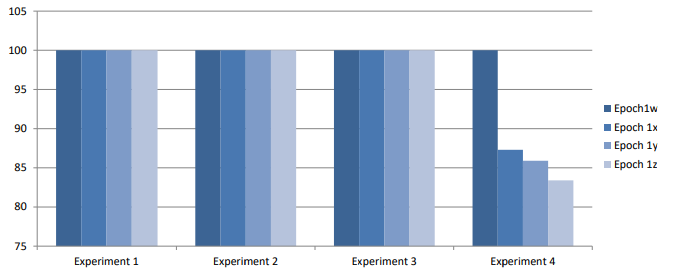
\includegraphics[width=14cm]{thesis/images/res01.PNG}\\
  \caption{WER, where w\<x\<y\<z are taken arbitrarily across the total
number of epochs} \label{fig_6_3_wer}
\end{figure}
